\documentclass[aspectratio=169,12pt]{beamer}
\usepackage[utf8]{inputenc}
\usepackage[T2A]{fontenc}
\usepackage[russian]{babel}
\usepackage{amsmath,amssymb}
\usepackage{booktabs}
\usepackage{graphicx}
\usepackage{xcolor}
\usepackage{multirow}
\usepackage{colortbl}
\usepackage{lmodern}

\definecolor{mipt}{RGB}{0,51,102}
\definecolor{miptmed}{RGB}{0,82,163}
\definecolor{miptlight}{RGB}{215,230,250}
\definecolor{accent}{RGB}{0,102,179}
\definecolor{good}{RGB}{0,115,56}
\definecolor{bad}{RGB}{185,10,10}
\definecolor{rowhl}{RGB}{228,240,255}
\definecolor{rowgray}{RGB}{245,246,250}

\usetheme{default}
\setbeamercolor{normal text}{fg=black!88}
\setbeamercolor{frametitle}{fg=white,bg=mipt}
\setbeamercolor{structure}{fg=mipt}
\setbeamercolor{block title}{fg=white,bg=miptmed}
\setbeamercolor{block body}{fg=black!88,bg=miptlight}
\setbeamercolor{block title alerted}{fg=white,bg=bad}
\setbeamercolor{block body alerted}{fg=black!85,bg=bad!8}
\setbeamercolor{item}{fg=accent}
\setbeamercolor{footline}{fg=mipt!60,bg=white}
\setbeamercolor{frametitle sep}{bg=accent}
\setbeamercolor{footline sep}{bg=mipt!20}

\setbeamertemplate{navigation symbols}{}

\setbeamerfont{normal text}{size=\small}
\setbeamerfont{frametitle}{size=\normalsize,series=\bfseries}
\setbeamerfont{block title}{size=\small,series=\bfseries}
\setbeamerfont{block body}{size=\small}
\setbeamerfont{footline}{size=\tiny}

\setlength{\leftmargini}{1.1em}
\setlength{\leftmarginii}{1.0em}

\setbeamertemplate{frametitle}{%
  \nointerlineskip
  \begin{beamercolorbox}[wd=\paperwidth,ht=2.2em,dp=0.4em,leftskip=1.0em,sep=0pt]{frametitle}%
    \usebeamerfont{frametitle}\vspace{0.5em}\insertframetitle
  \end{beamercolorbox}%
  \nointerlineskip
  \begin{beamercolorbox}[wd=\paperwidth,ht=1.5pt,dp=0pt]{frametitle sep}%
  \end{beamercolorbox}%
}

\setbeamertemplate{footline}{%
  \leavevmode
  \begin{beamercolorbox}[wd=\paperwidth,ht=0.5pt,dp=0pt]{footline sep}%
  \end{beamercolorbox}%
  \hbox{%
    \begin{beamercolorbox}[wd=0.73\paperwidth,ht=1.6em,dp=0.35em,leftskip=0.8em]{footline}%
      \usebeamerfont{footline}\color{mipt!60}%
      \vbox to 1.6em{\vfil%
        Vehicle Re-ID\ \textbullet\ Горбачев М.\,Д.\ \textbullet\ МФТИ 2026%
      \vfil}%
    \end{beamercolorbox}%
    \begin{beamercolorbox}[wd=0.27\paperwidth,ht=1.6em,dp=0.35em,rightskip=0.8em,right]{footline}%
      \usebeamerfont{footline}\color{mipt}%
      \vbox to 1.6em{\vfil\bfseries%
        \insertframenumber\,/\,\inserttotalframenumber%
      \vfil}%
    \end{beamercolorbox}%
  }%
}

\setbeamertemplate{itemize item}{%
  \color{accent}\raisebox{0.1ex}{\rule{0.48em}{0.48em}}}
\setbeamertemplate{itemize subitem}{%
  \color{accent!60}\raisebox{0.15ex}{\rule{0.36em}{0.36em}}}

\setbeamertemplate{itemize/enumerate body begin}{\small\setlength{\itemsep}{4pt}\setlength{\parsep}{0pt}\setlength{\parskip}{0pt}}
\setbeamertemplate{itemize/enumerate subbody begin}{\footnotesize\setlength{\itemsep}{2pt}}

\title[Vehicle Re-ID]{Исследование методов идентификации объектов\\
  при съёмке с разноракурсных камер наблюдения}
\subtitle{Vehicle Re-Identification: ResNet-50 / ResNet-101 vs ViT-Small on VeRi-776}
\author[Горбачев М.\,Д.]{Горбачев Максим Денисович\\[0.2em]
  {\small Научный руководитель: Назаров Алексей Николаевич}}
\institute[МФТИ]{МФТИ \textbullet\ ФРКТ \textbullet\ Группа М01-404}
\date{Май 2026}

\begin{document}

% ── 1. Титул ──────────────────────────────────────────────────────────────────
{
\setbeamercolor{background canvas}{bg=mipt}
\begin{frame}[plain]
  % Шапка: лого + институт
  \begin{center}
    
\includegraphics[height=1.6em]{../images/logo.png}\\[0.4em]
    {\fontsize{7}{9}\selectfont\color{miptlight}%
      Московский физико-технический институт (государственный университет)}\\[0.15em]
    % {\fontsize{6}{8}\selectfont\color{miptlight!70}%
    %   Физтех-школа радиотехники и компьютерных технологий}\\[0.1em]
    % {\fontsize{6}{8}\selectfont\color{miptlight!70}%
    %   Кафедра микропроцессорных технологий в интеллектуальных системах управления \textbullet\ 03.03.01 Прикладные математика и физика}
  \end{center}
  \vspace{0.3em}
  {\color{accent!50}\rule{\textwidth}{0.3pt}}\par
  \vspace{0.5em}
  % Название
  \begin{center}
    {\fontsize{16}{21}\selectfont\bfseries\color{white}%
    Исследование методов идентификации объектов\\[0.15em]
    при съёмке с разноракурсных камер наблюдения}\par
  \end{center}
  \vspace{1.2em}
  {\color{accent!50}\rule{\textwidth}{0.3pt}}\par
  \vspace{1.0em}
  % Автор / руководитель
  \begin{columns}[t,onlytextwidth]
    \column{0.5\textwidth}
    {\fontsize{7}{9}\selectfont\color{miptlight!60}Автор:}\\[0.2em]
    {\fontsize{8}{10}\selectfont\color{white}\textbf{Горбачев Максим Денисович}}\\[0.15em]
    {\fontsize{7}{9}\selectfont\color{miptlight!80}Студент группы М01-404}
    \column{0.5\textwidth}
    {\fontsize{7}{9}\selectfont\color{miptlight!60}Научный руководитель:}\\[0.2em]
    {\fontsize{8}{10}\selectfont\color{white}Назаров Алексей Николаевич}\\[0.15em]
    {\fontsize{7}{9}\selectfont\color{miptlight!80}Май 2026}
  \end{columns}
  \vspace{1.5em}
\end{frame}
}

% ── 2. Постановка задачи ──────────────────────────────────────────────────────
\begin{frame}{Постановка задачи}
  \begin{block}{Задача}
    Для запроса $q$ найти все изображения того же ТС в галерее $\mathcal{G}$
    с \emph{других} камер --- \textbf{без использования номерных знаков}
  \end{block}
  \vspace{0.6em}
  \begin{itemize}\setlength{\itemsep}{8pt}
    \item Построить $f_\theta\colon \mathcal{X}\to\mathbb{R}^d$ так, чтобы
          $D(f_\theta(q),f_\theta(g))\ll 1$ при $\mathrm{id}(g)=\mathrm{id}(q)$
    \item \textbf{Open-set}: тестовые ID не пересекаются с обучающими
    \item Протокол \emph{no-same-camera}
  \end{itemize}
\end{frame}

% ── 3. Сложности ──────────────────────────────────────────────────────────────
\begin{frame}{Сложности задачи}
  \begin{itemize}\setlength{\itemsep}{10pt}
    \item Смена ракурса и масштаба между камерами
    \item Вариативность освещения
    \item Окклюзии, низкое разрешение
    \item Domain shift между камерами
    \item Серийные ТС: нет уникальных биометрических признаков
    \item Номера недоступны: заляпаны, приватность, низкое разрешение
  \end{itemize}
\end{frame}

% ── 4. Датасет: статистика ────────────────────────────────────────────────────
\begin{frame}{Датасет VeRi-776: статистика}
  \begin{columns}[T,onlytextwidth]
    \column{0.52\textwidth}
    \begin{itemize}\setlength{\itemsep}{8pt}
      \item $\approx$50\,000 изображений
      \item \textbf{776 ТС}, \textbf{20 камер}
      \item Обучение: 575 ID --- 37\,746 изображений
      \item Query: 200 ID --- 1\,678 изображений
      \item Gallery: 200 ID --- 11\,579 изображений
      \item Протокол: \emph{single-query, no-same-camera}
    \end{itemize}
    \column{0.45\textwidth}
    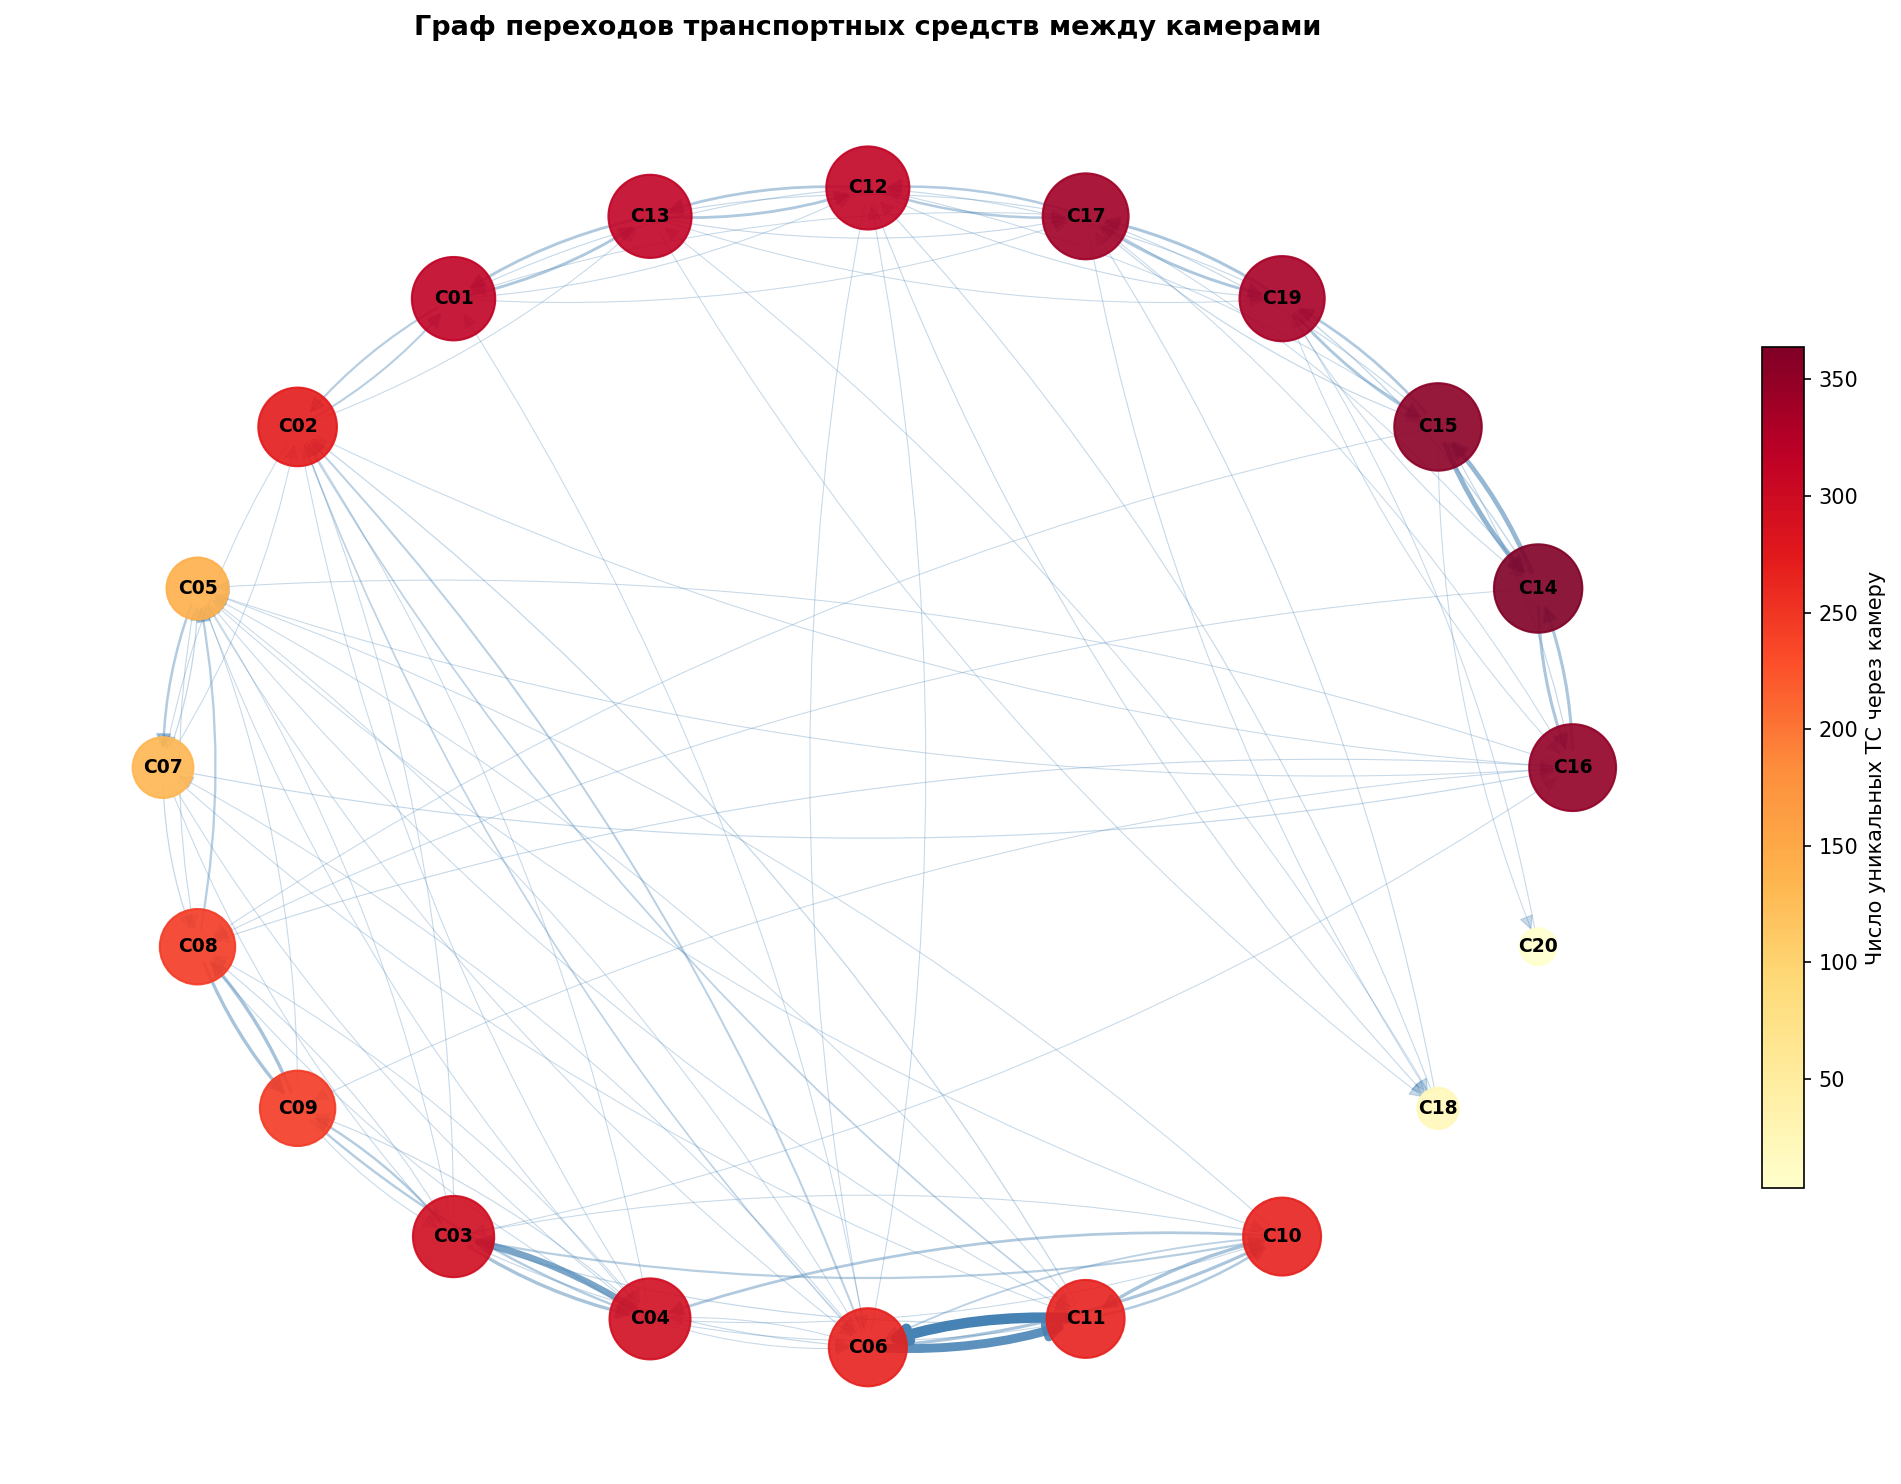
\includegraphics[width=\textwidth,height=0.65\textheight,keepaspectratio]{../images/camera_route_graph.png}
    {\footnotesize\centering Граф переходов между 20 камерами\par}
  \end{columns}
\end{frame}

% ── 5. Датасет: топология ─────────────────────────────────────────────────────
\begin{frame}{Датасет VeRi-776: топология маршрутов}
  \begin{itemize}\setlength{\itemsep}{10pt}
    \item 108 из 380 рёбер --- реальная дорожная сеть
    \item Среднее камер на маршруте: \textbf{8.9}
    \item C11~$\leftrightarrow$~C06: нагруженная пара (990 переходов)
    \item \textcolor{bad}{\textbf{C18}}: Rank-1 = 0--2.3\% у \emph{обеих} моделей --- проблема оборудования
  \end{itemize}
\end{frame}

% ── 6. Архитектура ResNet ─────────────────────────────────────────────────────
\begin{frame}{Архитектура: ResNet-50 / ResNet-101 + BNNeck}
  \begin{columns}[T,onlytextwidth]
    \column{0.52\textwidth}
    \begin{itemize}\setlength{\itemsep}{7pt}
      \item ResNet-50: \textbf{24.7M} пар., ImageNet-1k
      \item ResNet-101: \textbf{43.7M} пар., те же гиперпараметры
      \item Убран stride в \texttt{layer4}: feature map $16{\times}8$
      \item GAP $\to$ FC(2048) $\to$ \textbf{BNNeck}
      \item Вход: $256\times128$, эмбеддинг: $\mathbb{R}^{2048}$
    \end{itemize}
    \column{0.45\textwidth}
    \begin{block}{BNNeck}
      \small
      \textbf{До BN}: признаки для Triplet Loss\\[0.3em]
      \textbf{После BN + L2}: признаки для CE\\[0.3em]
      Разделение целей снижает конфликт
    \end{block}
    \vspace{0.5em}
    \begin{alertblock}{ResNet-101 $<$ ResNet-50}
      \small
      43.7M пар.\ при 37\,746 изображениях\\$\Rightarrow$ overfit
    \end{alertblock}
  \end{columns}
\end{frame}

% ── 7. Архитектура ViT-Small ──────────────────────────────────────────────────
\begin{frame}{Архитектура: ViT-Small + BNNeck}
  \begin{columns}[T,onlytextwidth]
    \column{0.50\textwidth}
    \begin{itemize}\setlength{\itemsep}{7pt}
      \item $224\times224 \to 196$ патчей $16\times16$
      \item Линейная проекция в $\mathbb{R}^{384}$
      \item CLS-токен --- глобальный дескриптор
      \item 12 блоков, 6 голов, \textbf{21.9M} пар.
      \item Pretrain: \textbf{ImageNet-21k} (14M изобр.)
    \end{itemize}
    \column{0.47\textwidth}
    \renewcommand{\arraystretch}{1.3}
    \begin{tabular}{lcc}
      \toprule
      & \textbf{RN-50} & \textbf{ViT-S} \\
      \midrule
      Параметры & 24.7M & 21.9M \\
      Эмбеддинг & 2048 & 384 \\
      Поле & локальное & глобальное \\
      Pretrain & 1k & \textbf{21k} \\
      \bottomrule
    \end{tabular}
    \vspace{0.5em}
    {\small$\mathrm{Attn}(Q,K,V)=\mathrm{softmax}\!\left(\dfrac{QK^\top}{\sqrt{d_k}}\right)\!V$}
  \end{columns}
\end{frame}

% ── 8. Функции потерь ─────────────────────────────────────────────────────────
\begin{frame}{Функции потерь}
  \begin{columns}[T,onlytextwidth]
    \column{0.50\textwidth}
    \begin{block}{Triplet Loss}
      \small
      $\mathcal{L}_t = \max\!\left(0,\, m + D(a,p) - D(a,n)\right)$\\[0.4em]
      Якорь $a$, позитив $p$, негатив $n$\\[0.2em]
      $m=0.3$, Hard mining, PK-семплинг
    \end{block}
    \column{0.46\textwidth}
    \begin{block}{Cross-Entropy + Label Smoothing}
      \small
      $\varepsilon = 0.1$\\[0.4em]
      Каждый ID = класс\\[0.2em]
      Сглаживание снижает самоуверенность
    \end{block}
  \end{columns}
  \vspace{0.8em}
  \begin{center}
  $\mathcal{L} = \mathcal{L}_{\mathrm{triplet}} + \mathcal{L}_{\mathrm{CE}}$
  \end{center}
\end{frame}

% ── 9. Гиперпараметры ────────────────────────────────────────────────────────
\begin{frame}{Гиперпараметры обучения}
  \begin{center}
  \renewcommand{\arraystretch}{1.4}
  \begin{tabular}{lcc}
    \toprule
    \textbf{Параметр} & \textbf{ResNet-50} & \textbf{ViT-Small} \\
    \midrule
    Оптимизатор & Adam & AdamW \\
    LR & $3.5\!\times\!10^{-4}$ & $1\!\times\!10^{-4}$ \\
    Weight decay & $5\!\times\!10^{-4}$ & $10^{-2}$ \\
    Эпохи & 120 & 50 \\
    Warmup & 5 & 10 \\
    Batch ($P\!\times\!K$) & $64\ (16\!\times\!4)$ & $48\ (12\!\times\!4)$ \\
    FP16 & да & да \\
    \bottomrule
  \end{tabular}
  \end{center}
  \vspace{0.4em}
  {\centering\small GPU: Google Colab T4 (16~GB)\par}
\end{frame}

% ── 10. Результаты ────────────────────────────────────────────────────────────
\begin{frame}{Результаты на VeRi-776}
  \begin{center}
  \renewcommand{\arraystretch}{1.4}
  \begin{tabular}{lccccc}
    \toprule
    \textbf{Модель} & \textbf{Rank-1} & \textbf{Rank-5} & \textbf{mAP}
                    & \textbf{Rank-1+RR} & \textbf{mAP+RR} \\
    \midrule
    ResNet-50  & 88.68 & 94.64 & 64.27 & 89.63 & 67.49 \\
    \rowcolor{rowgray}
    ResNet-101 & 86.65 & 93.86 & 57.67 & 87.96 & 60.08 \\
    \rowcolor{rowhl}
    \textbf{ViT-Small}
      & \textbf{90.05} & \textbf{96.25} & \textbf{69.41}
      & \textbf{91.90} & \textbf{74.49} \\
    \bottomrule
  \end{tabular}
  \end{center}
  \vspace{0.5em}
  \begin{itemize}
    \item ViT-Small лучше ResNet-50: Rank-1 \textbf{+1.4~п.п.}, mAP \textbf{+5.1~п.п.}
    \item ResNet-101 $<$ ResNet-50: overfit на малых данных
    \item Re-ranking: прирост ViT наибольший (\textbf{+5.1\%~mAP})
  \end{itemize}
\end{frame}

% ── 11. Эмбеддинги: PCA ───────────────────────────────────────────────────────
\begin{frame}{Геометрия эмбеддингов: PCA-визуализация}
  \begin{columns}[T,onlytextwidth]
    \column{0.48\textwidth}
    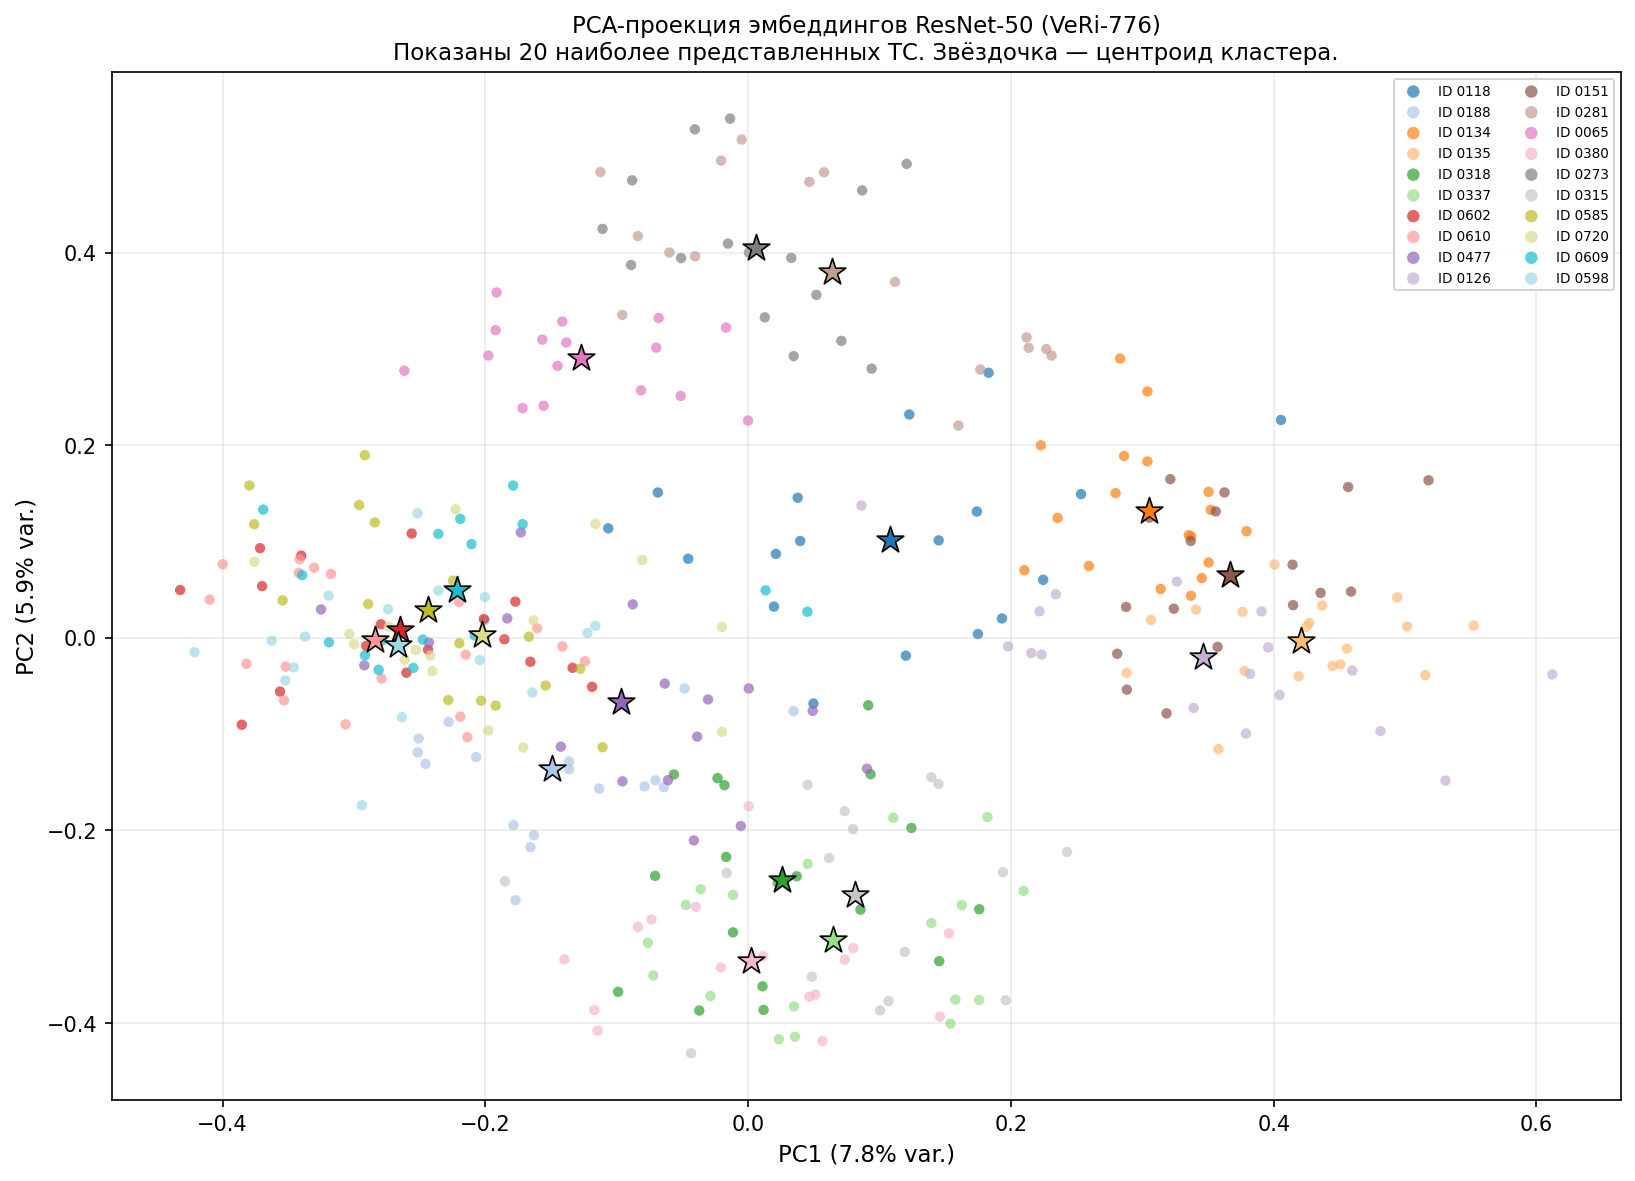
\includegraphics[width=\textwidth,height=0.6\textheight,keepaspectratio]{../images/pca_clusters_resnet50.png}
    {\centering\small ResNet-50: кластеры размыты\par}
    \column{0.48\textwidth}
    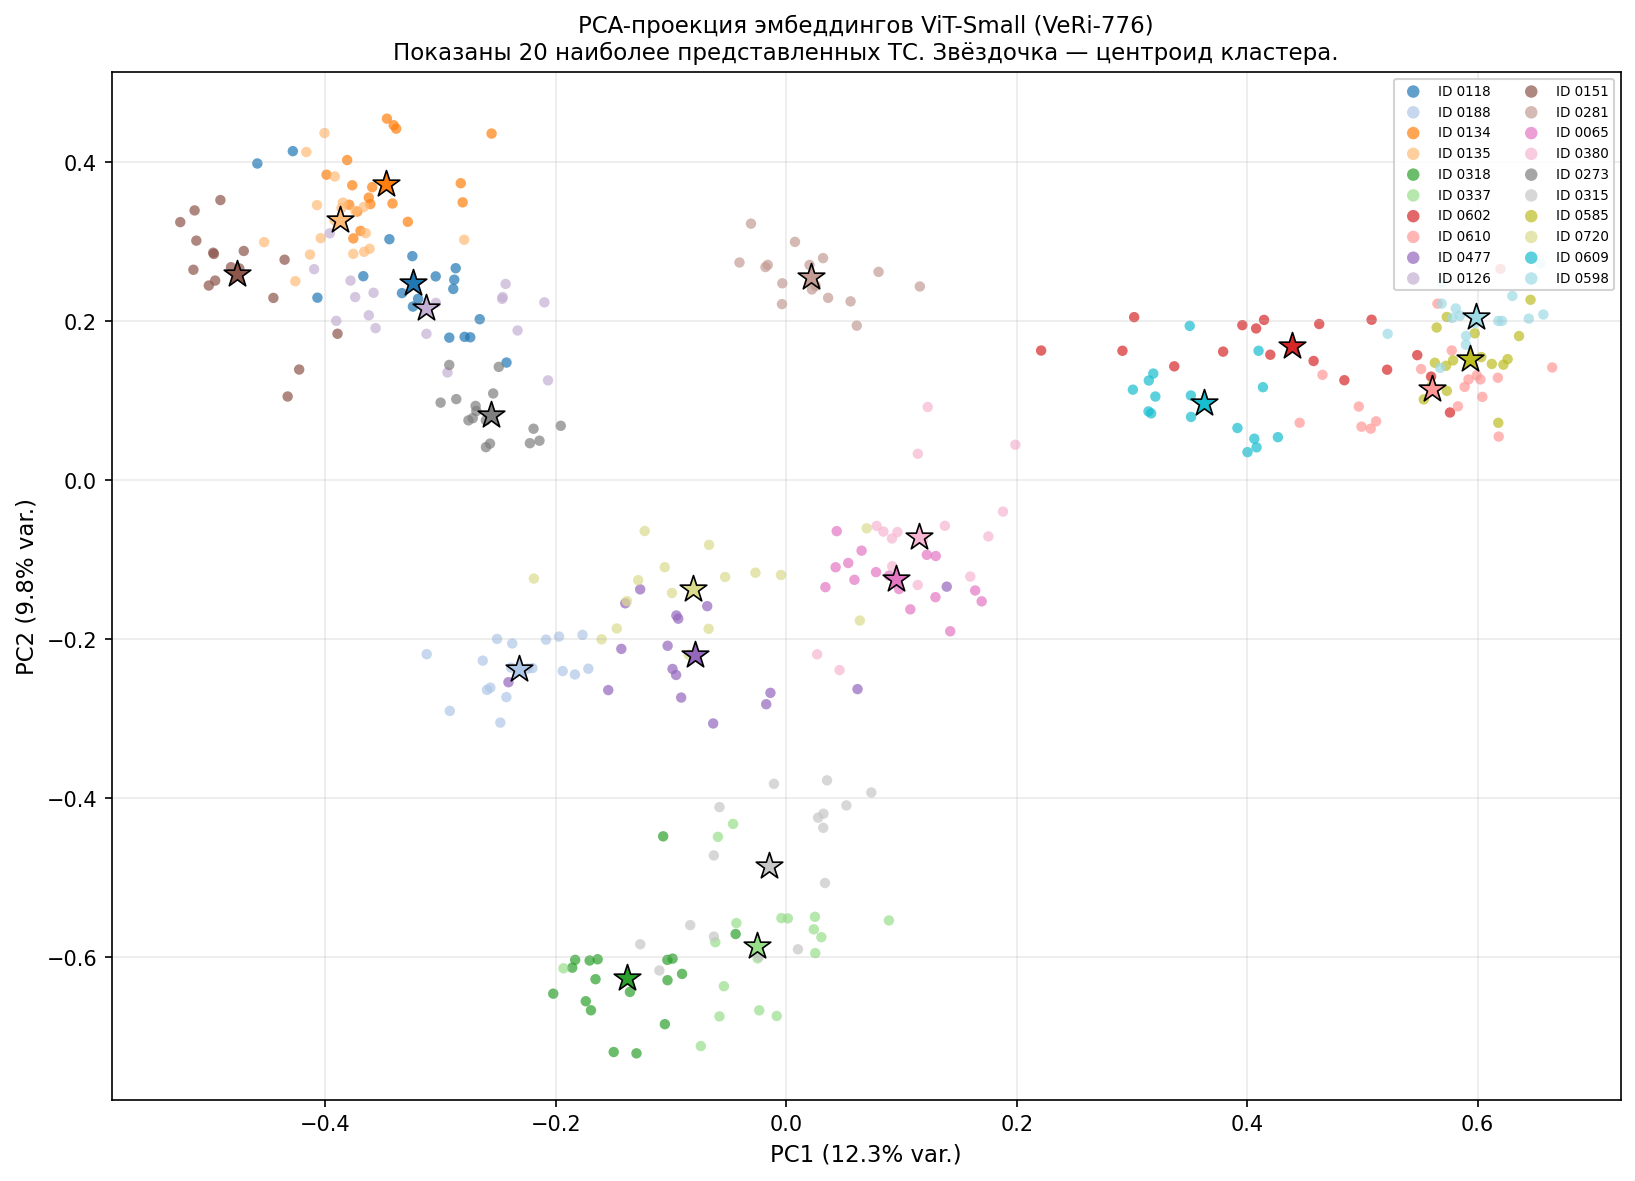
\includegraphics[width=\textwidth,height=0.6\textheight,keepaspectratio]{../images/pca_clusters_vit.png}
    {\centering\small ViT-Small: компактное разделение\par}
  \end{columns}
\end{frame}

% ── 12. Эмбеддинги: метрики ───────────────────────────────────────────────────
\begin{frame}{Геометрия эмбеддингов: метрики}
  \begin{center}
  \renewcommand{\arraystretch}{1.5}
  \begin{tabular}{lcc}
    \toprule
    \textbf{Метрика} & \textbf{ResNet-50} & \textbf{ViT-Small} \\
    \midrule
    Внутрикл.\ дисперсия & 0.434 & \textbf{0.247} ($\times$1.76 лучше) \\
    Межкластерное расст. & 0.787 & \textbf{1.212} ($\times$1.54 лучше) \\
    Коэф.\ силуэта & 0.024 & \textbf{0.260} ($\times$\textbf{10} лучше) \\
    \bottomrule
  \end{tabular}
  \end{center}
  \vspace{0.6em}
  {\centering\small Компактные кластеры ViT объясняют больший прирост от re-ranking\par}
\end{frame}

% ── 13. Карты внимания: метод ─────────────────────────────────────────────────
\begin{frame}{Карты внимания ViT-Small}
  \textbf{Метод агрегации:}
  \begin{itemize}\setlength{\itemsep}{8pt}
    \item Веса CLS-токена из \textbf{последних 4 блоков}
    \item Операция $\max$ по головам (не среднее)
    \item Перцентильная нормализация [5\%, 95\%]
  \end{itemize}
  \vspace{0.5em}
  \textbf{Почему не Attention Rollout?}\\[0.3em]
  {\small Перемножение 12 матриц $\to$ равномерное распределение; сигнал теряется}
\end{frame}

% ── 14. Карты внимания: результат ─────────────────────────────────────────────
\begin{frame}{Карты внимания ViT-Small: пример}
  \begin{columns}[c,onlytextwidth]
    \column{0.49\textwidth}
    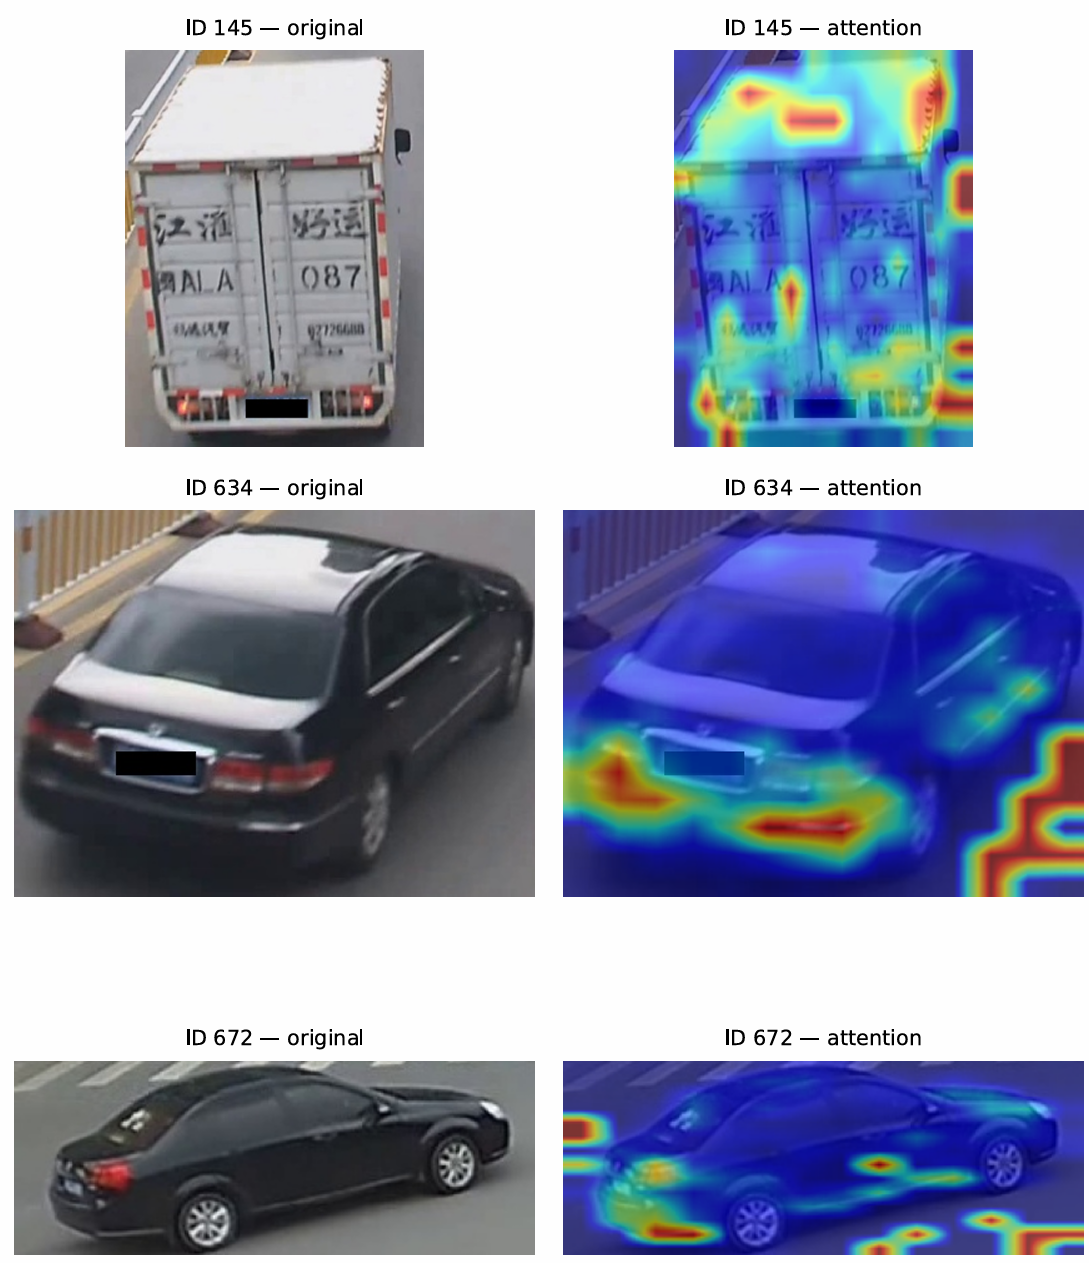
\includegraphics[width=0.85\textwidth]{../images/attention1.png}
    \column{0.49\textwidth}
    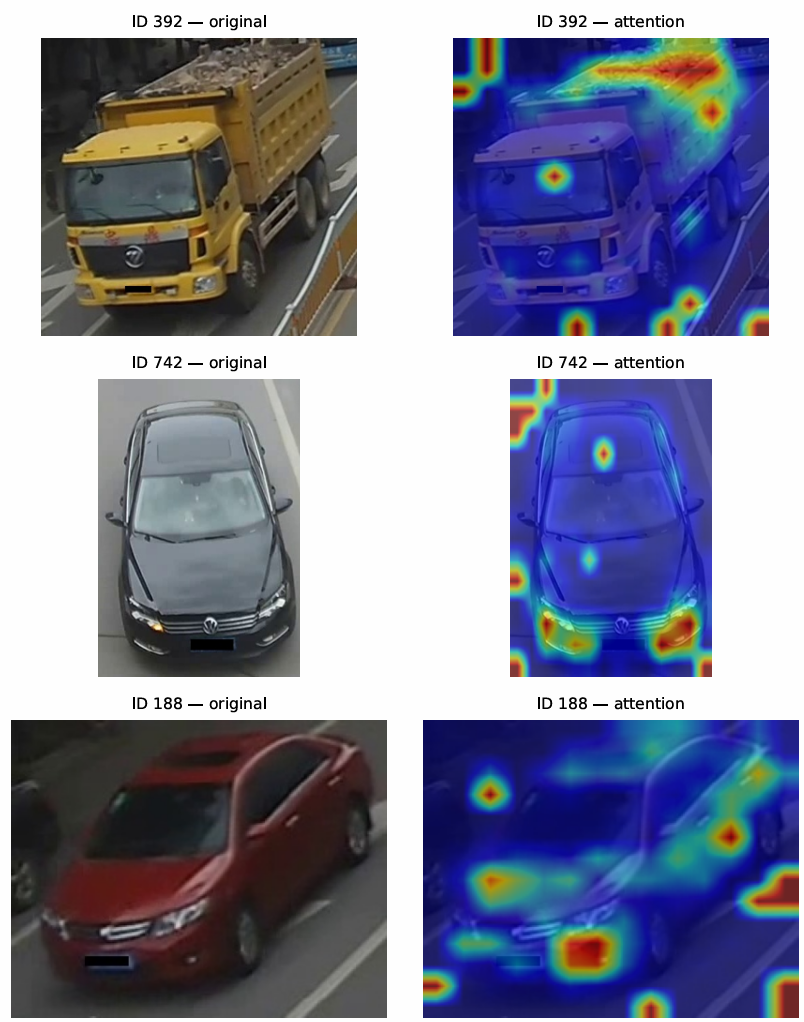
\includegraphics[width=0.85\textwidth]{../images/attention2.png}
  \end{columns}
\end{frame}

% ── 15. Качественные результаты: успех ───────────────────────────────────────
\begin{frame}{Качественные результаты: успешные случаи}
  \begin{center}
    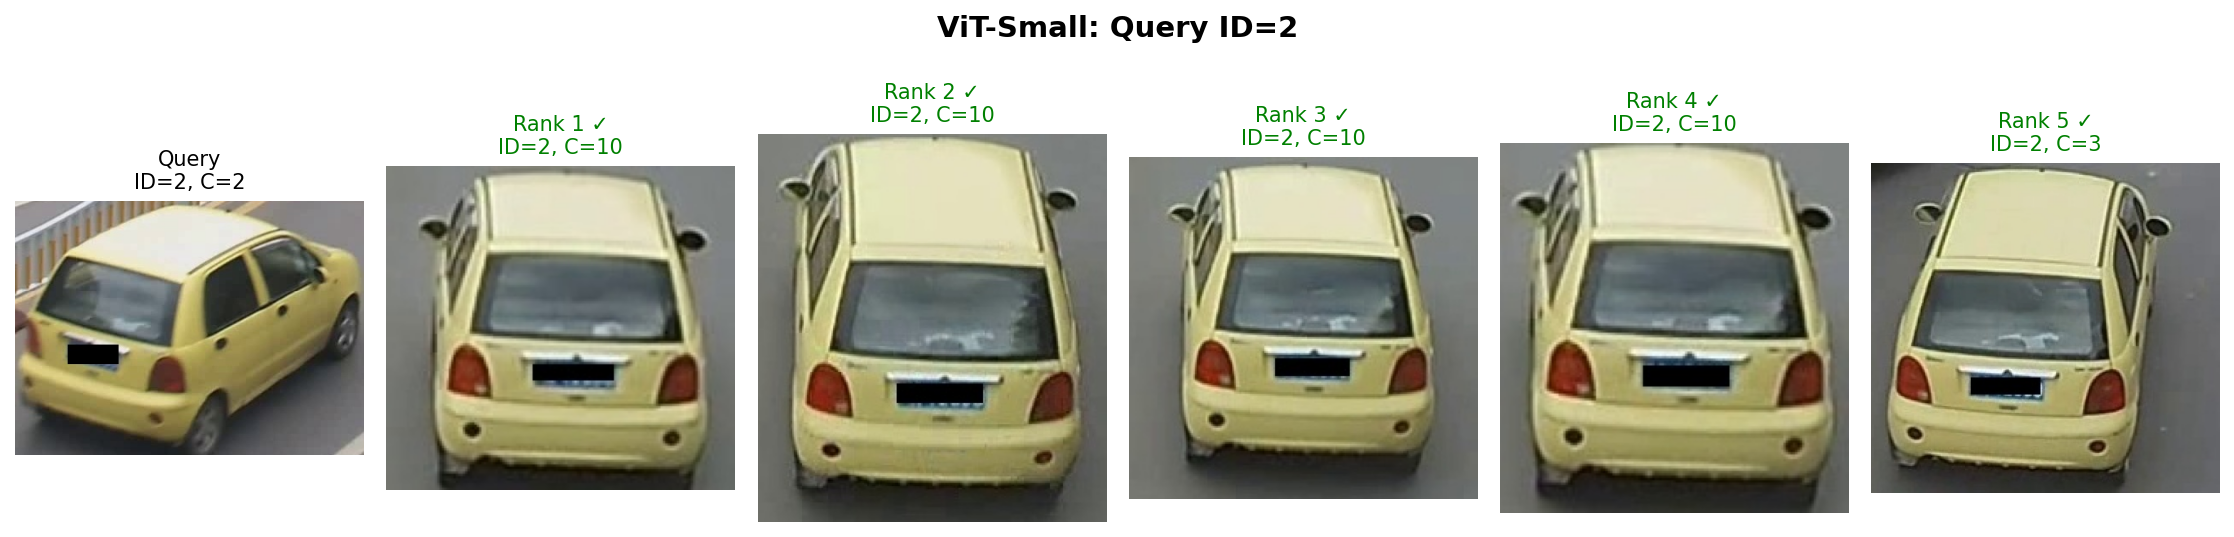
\includegraphics[width=0.95\textwidth]{../images/vit_example_1.png}
  \end{center}
  {\centering\small ViT-Small ID=2 (жёлтый хэтчбек): \textcolor{good}{\textbf{5/5}}\par}
  \vspace{0.4em}
  \begin{center}
    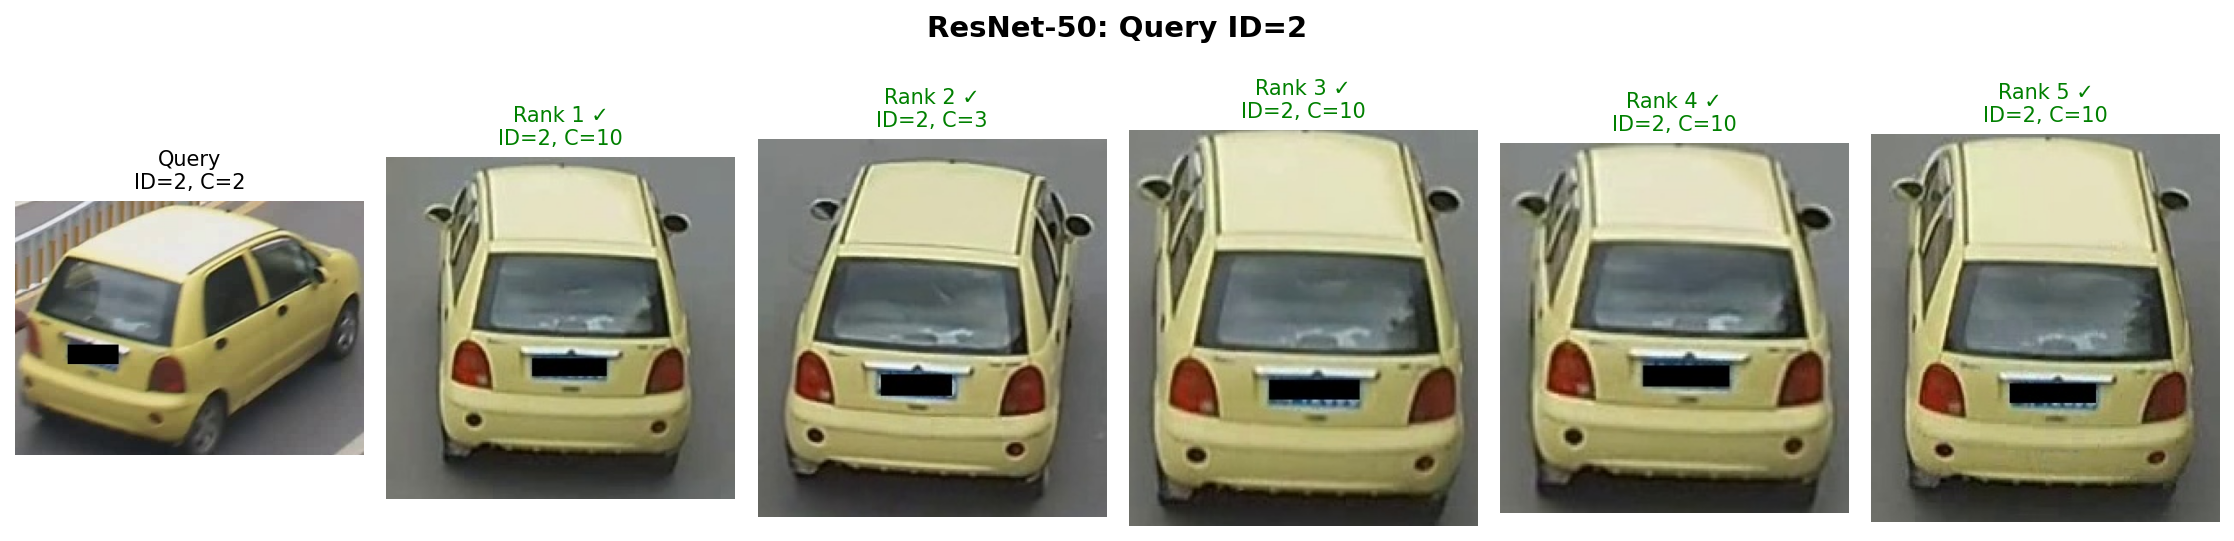
\includegraphics[width=0.95\textwidth]{../images/resnet50_example_1.png}
  \end{center}
  {\centering\small ResNet-50 ID=2: \textcolor{good}{\textbf{5/5}}\par}
\end{frame}

% ── 16. Качественные результаты: провал ───────────────────────────────────────
\begin{frame}{Качественные результаты: системный барьер}
  \begin{center}
    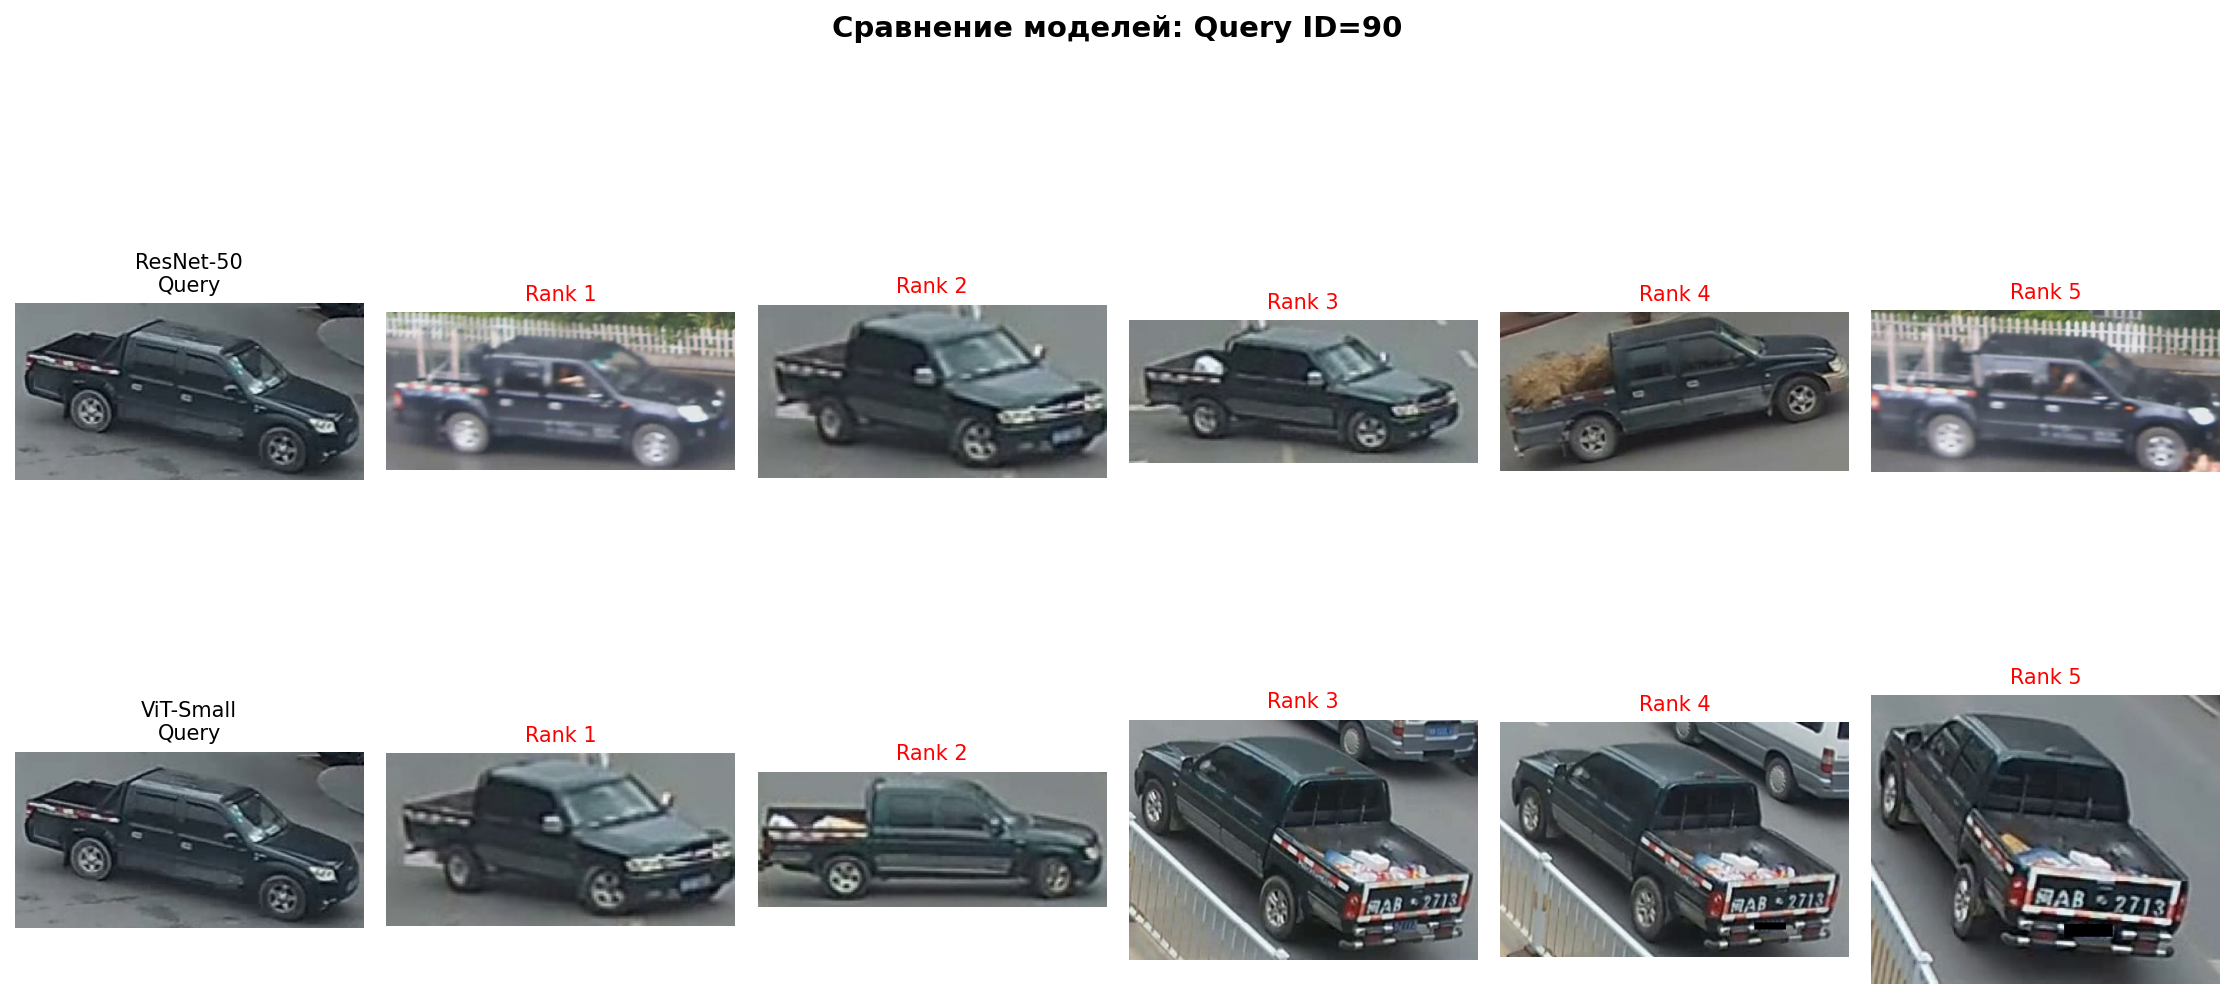
\includegraphics[width=0.95\textwidth,height=0.68\textheight,keepaspectratio]{../images/comparison_query_133.png}
  \end{center}
  {\centering\small\textcolor{bad}{\textbf{Чёрный внедорожник ID=90: обе модели 0/5}}\\
  Низкая контрастность --- схожие формы неразличимы\par}
\end{frame}

% ── 17. ViT на сложных запросах ───────────────────────────────────────────────
\begin{frame}{Преимущество ViT на сложных запросах}
  \begin{center}
    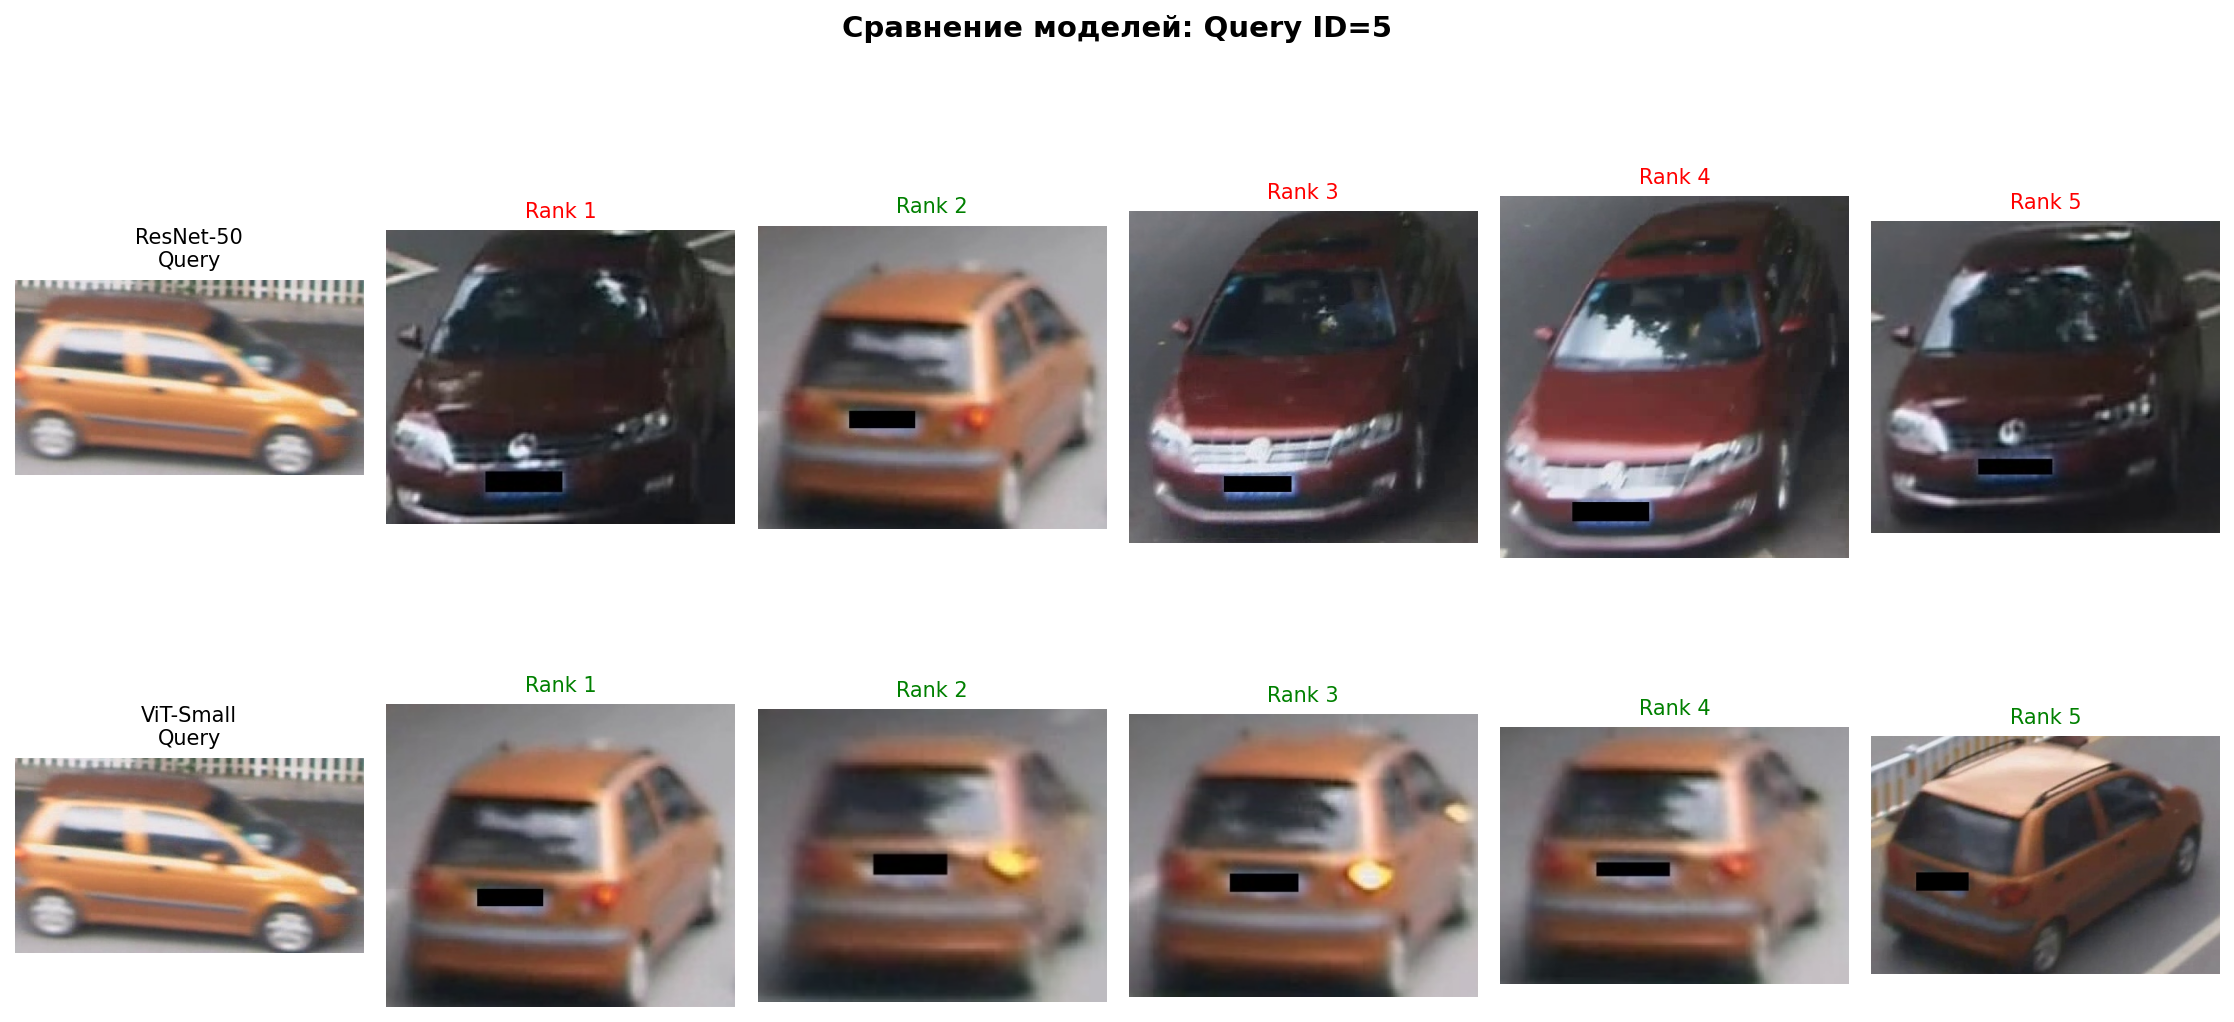
\includegraphics[width=0.88\textwidth]{../images/comparison_query_15.png}
  \end{center}
  {\centering\small
    Query ID=5 (оранжевый хэтчбек)\quad
    ResNet-50: \textcolor{bad}{\textbf{1/5}}\qquad
    ViT-Small: \textcolor{good}{\textbf{4/5}}\par}
  \vspace{0.3em}
  {\centering\footnotesize
    Глобальное внимание ViT связывает форму, цвет и текстуру одновременно\par}
\end{frame}

% ── 18. Пайплайн ─────────────────────────────────────────────────────────────
\begin{frame}{Пайплайн: YOLOv11n + ViT-Small + FAISS}
  \begin{columns}[T,onlytextwidth]
    \column{0.45\textwidth}
    \begin{enumerate}\setlength{\itemsep}{7pt}
      \item Кадр $\to$ \textbf{YOLOv11n} ($\approx$100~fps)
      \item Bbox $\to$ crop $224{\times}224$
      \item Crop $\to$ \textbf{ViT-Small} $\to$ $\mathbb{R}^{384}$
      \item Косинусный поиск \textbf{FAISS} ($\approx$1~мс / 10k)
    \end{enumerate}
    \vspace{0.5em}
    {\small%
    GT-кроп: Rank-1 = \textbf{90.05\%}\\
    YOLO-кроп: Rank-1 = \textbf{85.88\%}\\
    \textcolor{bad}{Разрыв $-4.17$~п.п.}}
    \column{0.52\textwidth}
    \vspace{0.5em}
    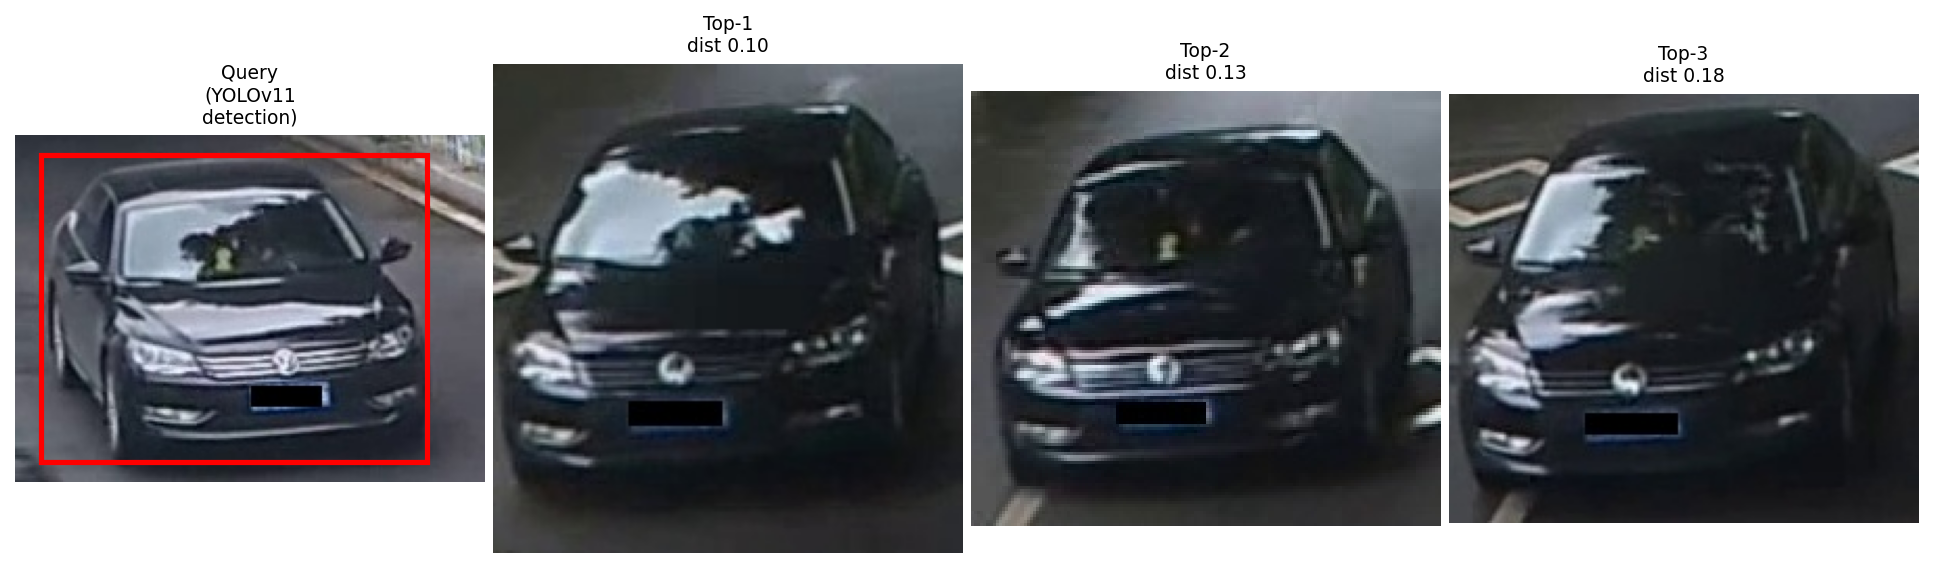
\includegraphics[width=\textwidth]{../images/yolo_reid_demo.png}
    {\centering\small YOLO-bbox + топ-3 из галереи\par}
  \end{columns}
\end{frame}

% ── 19. Тепловая карта ────────────────────────────────────────────────────────
\begin{frame}{Тепловая карта Rank-1 по парам камер}
  \begin{center}
    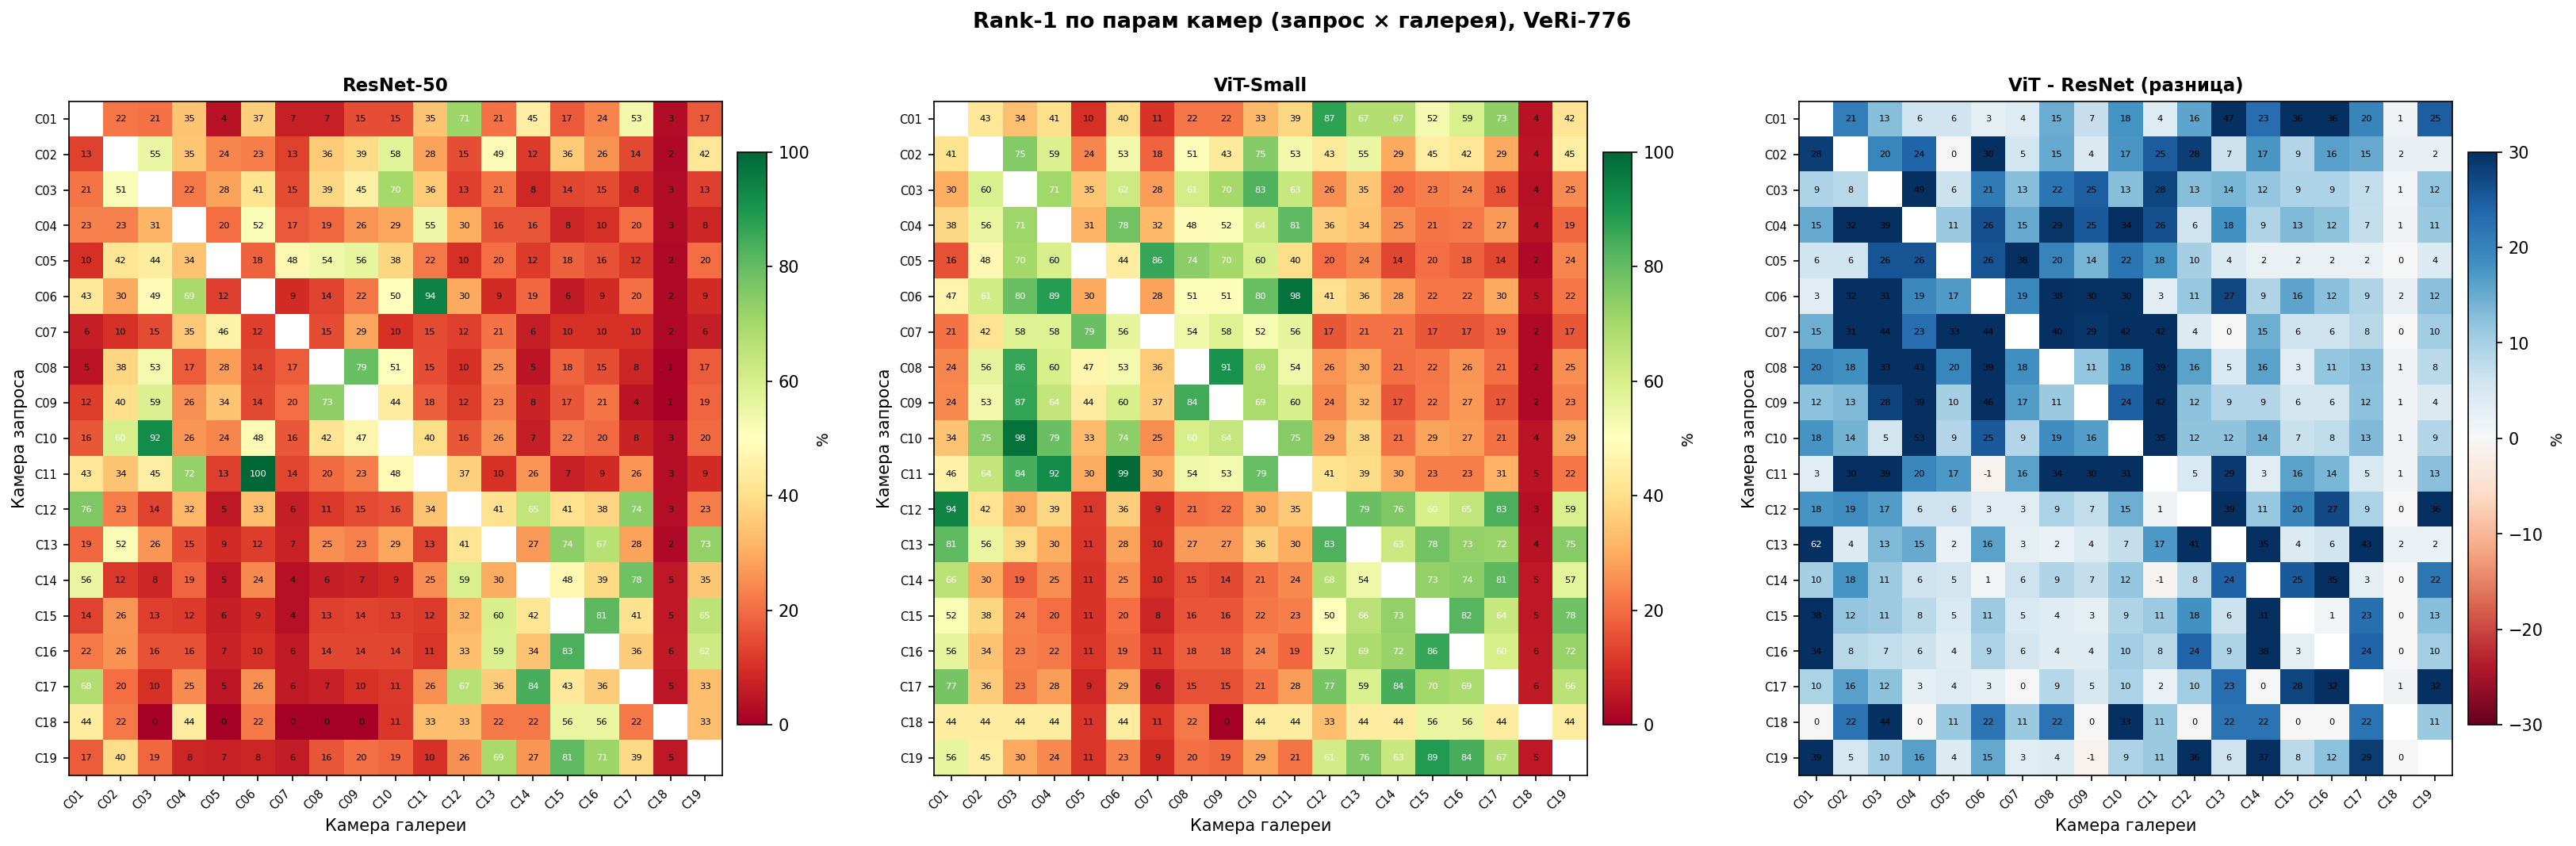
\includegraphics[width=0.88\textwidth,height=0.55\textheight,keepaspectratio]{../images/camera_heatmap_comparison.png}
  \end{center}
  \begin{columns}[T,onlytextwidth]
    \column{0.48\textwidth}
    {\small\textcolor{good}{\textbf{C11$\to$C06}}: ResNet 100\%, ViT 98.9\%\\
    ViT лучше на 94.2\% ненулевых пар}
    \column{0.48\textwidth}
    {\small\textcolor{bad}{\textbf{C18}}: Rank-1 = 0--2.3\% у обеих моделей\\
    Суммарные метрики это не выявляют}
  \end{columns}
\end{frame}

% ── 20. Расстояние Махаланобиса ───────────────────────────────────────────────
\begin{frame}{Негативный результат: расстояние Махаланобиса}
  \textbf{Гипотеза:} $d_M(x,y) = \sqrt{(x-y)^\top\Sigma^{-1}(x-y)}$ должен улучшить поиск, учитывая корреляции признаков
  \vspace{0.5em}
  \begin{center}
  \renewcommand{\arraystretch}{1.4}
  \begin{tabular}{lccc}
    \toprule
    & \textbf{L2} & \textbf{Mahala.} & $\Delta$ \\
    \midrule
    ResNet-50 mAP & 64.27 & 64.55 & $+0.28$ \\
    ViT-Small mAP  & 69.41 & 38.43 & \textcolor{bad}{$\mathbf{-30.98}$} \\
    \bottomrule
  \end{tabular}
  \end{center}
  \vspace{0.5em}
  \begin{alertblock}{Причина}
    \small
    После L2-нормализации эмбеддинги на сфере $\mathcal{S}^{383}$.
    $\Sigma^{-1}$ описывает эллипсоид в $\mathbb{R}^{384}$ --- разрушает угловые отношения.
    Для L2-нормированных векторов косинусное расстояние оптимально.
  \end{alertblock}
\end{frame}

% ── 21. Заключение: что сделано ───────────────────────────────────────────────
\begin{frame}{Заключение: что реализовано}
  \begin{columns}[T,onlytextwidth]
    \column{0.50\textwidth}
    \begin{itemize}\setlength{\itemsep}{6pt}
      \item ResNet-50, ResNet-101, ViT-Small + BNNeck
      \item K-reciprocal re-ranking
      \item PCA, силуэт, дисперсия эмбеддингов
      \item Тепловая карта по 20 камерам
      \item Карты внимания ViT-Small
      \item End-to-end: YOLOv11 + ViT + FAISS
    \end{itemize}
    \column{0.47\textwidth}
    \renewcommand{\arraystretch}{1.3}
    \begin{tabular}{lcc}
      \toprule
      \textbf{Модель} & \textbf{Rank-1} & \textbf{mAP+RR} \\
      \midrule
      ResNet-50 & 88.68 & 67.49 \\
      ResNet-101 & 86.65 & 60.08 \\
      \rowcolor{rowhl}\textbf{ViT-Small} & \textbf{90.05} & \textbf{74.49} \\
      \bottomrule
    \end{tabular}
  \end{columns}
\end{frame}

% ── 22. Заключение: выводы ────────────────────────────────────────────────────
\begin{frame}{Заключение: выводы и перспективы}
  \begin{columns}[T,onlytextwidth]
    \column{0.50\textwidth}
    \textbf{Выводы:}
    \begin{itemize}\setlength{\itemsep}{6pt}
      \item ViT-Small лучший: Rank-1 90.1\%, mAP 69.4\%
      \item ResNet-101 $<$ ResNet-50: глубина без нового pretrain не помогает
      \item Силуэт ViT в \textbf{10$\times$} лучше
      \item C18: системная проблема камеры
      \item Махаланобис на гиперсфере ломает геометрию ($-31\%$ mAP)
    \end{itemize}
    \column{0.46\textwidth}
    \textbf{Перспективы:}
    \begin{itemize}\setlength{\itemsep}{6pt}
      \item ViT-Base / DINOv2 / CLIP-ReID
      \item Multi-object tracking (ByteTrack)
      \item UDA на российских датасетах
    \end{itemize}
  \end{columns}
\end{frame}

% ── 23. Спасибо ───────────────────────────────────────────────────────────────
{
\setbeamercolor{background canvas}{bg=mipt}
\begin{frame}[plain]
  \vspace{2em}
  \begin{center}
    {\LARGE\bfseries\color{white} Спасибо за внимание!}\\[0.8em]
    {\large\color{miptlight} Вопросы?}
  \end{center}
\end{frame}
}

\end{document}
